\documentclass[12pt,a4paper]{article}

\usepackage{fancyhdr, titlesec}
\usepackage{geometry, graphicx, tikz}
\usepackage{pdfprivacy, xcolor}
\usepackage{hyperref}

\hypersetup{
	pdftitle={Git and GitHub Hands-On Guide},
	pdfauthor={Nicolás Aguado},
	pdfsubject={},
	pdfproducer={},
	pdfcreator={},
	pdfdisplaydoctitle=true,
	colorlinks,
	linkcolor={blue!20!black},
	citecolor={blue!20!black},
	urlcolor={blue!20!black}
}

% Set page geometry
\geometry{left=1in, right=1in, top=1in, bottom=1in}

% Document Title
\title{Git \& GitHub Hands-On}
\author{Nicolás Aguado}
\date{\today}

% Add a subtitle
\newcommand{\subtitle}[1]{
	\large\textit{#1}
}

% Setup headers
\usetikzlibrary{arrows.meta}
\pagestyle{fancy}
\fancyhf{}
\renewcommand{\headrulewidth}{0.4pt}
\setlength{\headheight}{14.5pt}
\fancyhead[L]{Git \& GitHub \emph{Hands-On}}
\fancyhead[R]{\thepage}

\begin{document}
	
	% Cover Page
	\begin{titlepage}
		\centering
		\vspace*{4cm}
		\hrule \vspace{1cm}
		\Huge\textbf{Git \& GitHub \\ \emph{Hands-On}}\\[0.5cm]
		\subtitle{An opinionated guide}\\[1cm]
		\hrule \vspace{1cm}
		\large{\textbf{Nicolás Aguado} \\ nico@nico.eus}\\[0.5cm]
		\large{\today}
		\vfill
		\begin{center}
			
			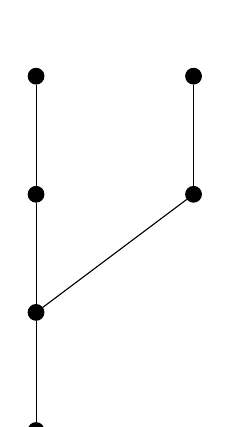
\begin{tikzpicture}[
				node/.style={circle, draw, fill=black, inner sep=2pt}
				]
				
				% Define nodes
				\node[node] (A) at (0, 0) {};
				\node[node] (B) at (0, -1.5) {};
				\node[node] (C) at (0, -3) {};
				\node[node] (D) at (2, -1.5) {};
				\node[node] (E) at (2, 0) {};
				\node[node] (F) at (0, -4.5) {};
				
				% Draw edges
				\draw[-] (A) -- (B);
				\draw[-] (B) -- (C);
				\draw[-] (D) -- (C);
				\draw[-] (E) -- (D);
				\draw[-] (F) -- (C);
				
			\end{tikzpicture}
			
			
		\end{center}
		\vspace{2cm}
		\vfill
	\end{titlepage}
	
	\newpage
	
	\begin{enumerate}
		\item 
		Motivation
		
		\vspace{2cm}
		

		
\begin{tikzpicture}
			% Draw the first file
			\fill[white] (0,0) rectangle (3,4);
			\draw[thick] (0,0) -- (0,4) -- (3,4) -- (3,0) -- cycle;
			
			% Folded corner of the first file
			\fill[gray!20] (2.2,4) -- (3,4) -- (3,3.2) -- cycle;
			\draw[thick] (2.2,4) -- (3,4) -- (3,3.2);
			
			% Lines to represent text in the first file
			\draw[thick] (0.5,3.3) -- (2.5,3.3);
			\draw[thick] (0.5,2.8) -- (2.5,2.8);
			\draw[thick] (0.5,2.3) -- (2.5,2.3);
			\draw[thick] (0.5,1.8) -- (1.8,1.8);
			
			% Draw the second file slightly offset
			\fill[white] (1,-0.5) rectangle (4,3.5);
			\draw[thick] (1,-0.5) -- (1,3.5) -- (4,3.5) -- (4,-0.5) -- cycle;
			
			% Folded corner of the second file
			\fill[gray!20] (3.2,3.5) -- (4,3.5) -- (4,2.7) -- cycle;
			\draw[thick] (3.2,3.5) -- (4,3.5) -- (4,2.7);
			
			% Lines to represent text in the second file
			\draw[thick] (1.5,2.8) -- (3.5,2.8);
			\draw[thick] (1.5,2.3) -- (3.5,2.3);
			\draw[thick] (1.5,1.8) -- (3.5,1.8);
			\draw[thick] (1.5,1.3) -- (2.8,1.3);
			
			% Draw the third file slightly more offset
			\fill[white] (2,-1) rectangle (5,3);
			\draw[thick] (2,-1) -- (2,3) -- (5,3) -- (5,-1) -- cycle;
			
			% Folded corner of the third file
			\fill[gray!20] (4.2,3) -- (5,3) -- (5,2.2) -- cycle;
			\draw[thick] (4.2,3) -- (5,3) -- (5,2.2);
			
			% Lines to represent text in the third file
			\draw[thick] (2.5,2.3) -- (4.5,2.3);
			\draw[thick] (2.5,1.8) -- (4.5,1.8);
			\draw[thick] (2.5,1.3) -- (4.5,1.3);
			\draw[thick] (2.5,0.8) -- (3.8,0.8);
			
			% Draw the open envelope icon to the right, spaced double the distance to the right
			% Draw the main rectangle for the envelope
			\fill[white] (10,0) rectangle (13,2);
			\draw[thick] (10,0) -- (10,2) -- (13,2) -- (13,0) -- cycle;
			
			
			% Draw the bottom triangle of the envelope pointing down
			\draw[thick] (10,2) -- (11.5,1.2) -- (13,2);
			
		\end{tikzpicture}

		
		\vspace{2cm}
		
			
		\textbf{Git} \footnote{\href{https://git-scm.com/}{\texttt{git-scm.com}}} \footnote{Explorer Association, Notepad as Default Editor} \\ \textbf{G}lobal \textbf{I}nformation \textbf{T}racker \\ \textbf{G}oddamn \textbf{I}diotic \textbf{T}ruckload of shit
		
		\vspace{1cm}
		\textbf{Source code} version control - Based on \emph{commits} - Scope: Only text files
		
		\newpage 
		
		\item Working Tree (Checkout, Commit) \\ \href{https://github.com/nicoGHO/workingtree}{\texttt{nicoGHO/workingtree}}
		\footnote{\texttt{git log}}
		\footnote{\texttt{tail -f <file>}}
		\footnote{\texttt{git checkout <hash|master>}}
		\footnote{\texttt{git add <file|pattern>}}
		\footnote{\texttt{git commit -m <msg>}}
		\vspace{1cm}
		
		
		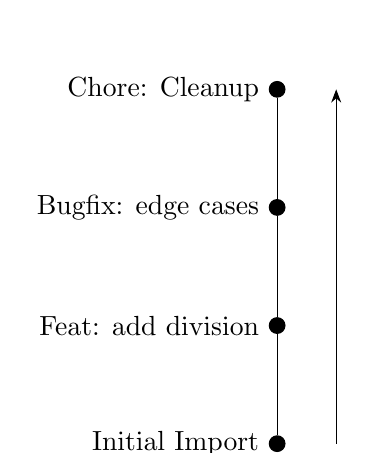
\begin{tikzpicture}[
			node/.style={circle, draw, fill=black, inner sep=2pt}
			]
			
			% Define nodes
			\node[node, label=left:Chore: Cleanup] (A) at (0, 0) {};
			\node[node, label=left:Bugfix: edge cases] (B) at (0, -1.5) {};
			\node[node, label=left:Feat: add division] (C) at (0, -3) {};
			\node[node, label=left:Initial Import] (F) at (0, -4.5) {};
			
			% Draw edges
			\draw[-] (A) -- (B);
			\draw[-] (B) -- (C);
			\draw[-] (F) -- (C);
			
			% Draw arrow
			\draw[-{Stealth[black]}] (0.75, -4.5) -- (0.75,0);
			
		\end{tikzpicture}
		
		\newpage
		\item Git Graphical Clients \\ Environment Setup
	
	
		\vspace{1cm}
		
		Setup Environment Variables \\
		Microsoft VSCode \footnote{\href{https://code.visualstudio.com/}{\texttt{code.visualstudio.com}}}, GitKraken \footnote {\href{https://www.gitkraken.com/}{\texttt{gitkraken.com}}}
		
		\vspace{1cm}
		\href{https://github.com/nicoGHO/workingtree}{\texttt{nicoGHO/workingtree}}
		
		\newpage 
		\item Good practices with projects
		\begin{itemize}
			\item Use descriptive commit messages (feat, bugfix, chore)
			\item Use .gitignore (Minimal per folder, granularity)
			\item Do relatively small commits (Max. 100-200 lines)
			\item Dot (.) files are usually configuration files - do not touch them
		\end{itemize}
		
		
		\newpage
		\item Branches \footnote{Cuidado en VSCode con el modo \emph{detached}!} \\ Tags
		
		\vspace{2cm}
		
		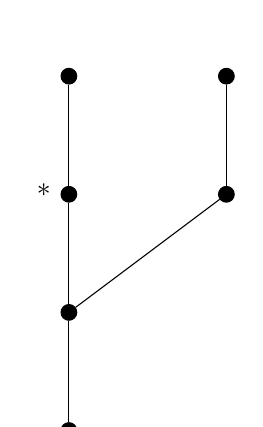
\begin{tikzpicture}[
			node/.style={circle, draw, fill=black, inner sep=2pt}
			]
			
			% Define nodes
			\node[node] (A) at (0, 0) {};
			\node[node, label=left:*] (B) at (0, -1.5) {};
			\node[node] (C) at (0, -3) {};
			\node[node] (D) at (2, -1.5) {};
			\node[node] (E) at (2, 0) {};
			\node[node] (F) at (0, -4.5) {};
			
			% Draw edges
			\draw[-] (A) -- (B);
			\draw[-] (B) -- (C);
			\draw[-] (D) -- (C);
			\draw[-] (E) -- (D);
			\draw[-] (F) -- (C);
			
		\end{tikzpicture}
		
		\vspace{3cm}
		Merge, Merge Conflicts \\ \href{https://github.com/nicoGHO/branches}{\texttt{nicoGHO/branches}}
		\vspace{1cm}
		
		\begin{tikzpicture}[
			node/.style={circle, draw, fill=black, inner sep=2pt}
			]
			
			% Define nodes
			\node[node] (A) at (0, 0) {};
			\node[node] (B) at (0, -3) {};
			\node[node] (C) at (0, -4.5) {};
			\node[node] (D) at (2, -3) {};
			\node[node] (E) at (2, 0) {};
			\node[node] (F) at (0, -6) {};
			\node[node] (G) at (4, -1.5) {};
			\node[node] (H) at (2, -1.5) {};
 			
			% Draw edges
			\draw[-] (A) -- (B);
			\draw[-] (B) -- (C);
			\draw[-] (D) -- (C);
			\draw[-] (E) -- (H);
			\draw[-] (D) -- (H);
			\draw[-] (F) -- (C);
			\draw[-] (D) -- (G);
			
		\end{tikzpicture}
		
		
		\newpage
		\item Good practices with branches
		\begin{itemize}
			\item Protected \textbf{stable} master branch
			
			\item One branch per feature / person / organization
			
			\item Merges done with affected coder(s) present
		\end{itemize}
		
		
		\vspace{10cm}
		Rebase, Cherry-Pick

		
		\newpage
		\item Git in the Cloud (GitHub) \footnote{\texttt{git config --global user.name "John Doe"}} \footnote{\texttt{git config --global user.email johndoe@example.com}} \\ Origin (Clone, Push, Pull) \footnote{\texttt{git clone <remote url>}} \footnote{\texttt{git push (<origin>)}} \\ Permissions for GUIs (Private Clone, Contribute) \footnote{En Linux: \texttt{git config --global credential.credentialStore cache}}
		
		
		\vspace{1cm}
		\href{https://github.com/nicoGHO/pushpull}{\texttt{nicoGHO/pushpull}}
		
		\vspace{7cm}
		Conflicts when pushing and pulling - People working at same time on \textbf{same branch}
		
		\vspace{3cm}
		
		\begin{tikzpicture}[
			node/.style={circle, draw, fill=black, inner sep=2pt}
			]
			
			% Define nodes
			\node[node] (B) at (0, -1.5) {};
			\node[node] (C) at (0, -3) {};
			\node[node] (F) at (0, -4.5) {};
			\node[node] (G) at (1.5, 0) {};
			
			% Draw edges
			\draw[-] (0,0) -- (B);
			\draw[-] (B) -- (C);
			\draw[-] (F) -- (C);
			\draw[-] (B) -- (G);
			
			
		\end{tikzpicture}
		
				
		\newpage
		\item Visualization (Code, README) \\ Commits \\ Network Graph \\ Issues \\ Projects
		
		\vspace{1cm}
		\href{https://github.com/nextcloud/server}{\texttt{nextcloud/server}}
		
		\newpage
		\item Pull Requests \\ Permission-regulated
		
		\vspace{1cm}
		\href{https://github.com/nicoGHO/pullrequests}{\texttt{nicoGHO/pullrequests}}
		
		\newpage
		\item Submodules \\
		Adding \footnote{\texttt{git submodule add <repository-url> <path>}}, Updating \footnote{\texttt{git submodule update (--init --recursive)|(--remote)}} (\emph{Commit-based} \texttt{.gitmodules}) \\ Cloning \footnote{\texttt{git clone --recursive <project url>}} \\ Easier if inmutable
		
		\vspace{1cm}
		\href{https://github.com/nicoGHO/submodules}{\texttt{nicoGHO/submodules}}
		
		\vspace{2cm}
		
		\begin{tikzpicture}[
			node/.style={circle, draw, fill=black, inner sep=2pt}
			]
			
			% Define nodes
			\node[node] (A) at (0, 0) {};
			\node[node] (B) at (0, -1.5) {};
			\node[node] (C) at (0, -3) {};
			\node[node] (F) at (0, -4.5) {};
			
			\node[node] (B2) at (4, -1.5) {};
			\node[node, label=right:chore: update submodule] (C2) at (4, -3) {};
			\node[node] (F2) at (4, -4.5) {};
			
			% Draw edges
			\draw[-] (A) -- (B);
			\draw[-] (B) -- (C);
			\draw[-] (F) -- (C);
			
			\draw[-] (B2) -- (C2);
			\draw[-] (F2) -- (C2);
			
			\draw[-{Stealth[black]}] (C) -- (C2);	
			
		\end{tikzpicture}
		
		\newpage
		\item Summary
		
		\vspace{1cm}
		
		To start:
		
		\texttt{git clone --recursive <project url>}
		
		To edit:
		\begin{itemize}
			\item Create branch or checkout one
			\item Edit, commit
			\item ¿Push?
			\item Edit, commit
			\item Submodule has updated? Run commands
			\item Edit, commit
			\item Issue arises and not your responsability? Document it
			\item Edit, commit
			\item Pull request for merging into staging
			\item Ask your local wizard for merge
			\item Repeat
		\end{itemize}
		
		If something breaks:
		
		Do not be afraid to use the terminal! Rollbacks are used every day!
		
		\vspace{3cm}
		¡Use git and \textbf{learn by fighting against it}!
		
		\vspace{2cm}
		These are some extra topics left as an exercise to the reader
		\begin{itemize} 
			\item Git LFS
			\item Multi-Remote Work
			\item Revert Pushed Commits
			\item Several Stable Branches (prod, pre, dev)
			\item Commit Stashes
			\item Automatic Deployments (CI/CD)
		\end{itemize}
		
		
		
	\end{enumerate}
	
	
\end{document}
